\documentclass[12pt]{book}

\usepackage{amssymb}
\usepackage{amsmath}
\usepackage{amsthm}
\usepackage{amsfonts}
\usepackage[spanish]{babel}
\usepackage[utf8]{inputenc}
\usepackage[T1]{fontenc}
\usepackage{graphicx}
\usepackage[figuresright]{rotating}
\usepackage{subfigure}
\usepackage{epstopdf}
\usepackage{float}
\usepackage{natbib}
\usepackage[skip=10pt,labelfont=bf,labelsep=period]{caption}
\usepackage[paperwidth=215mm,paperheight=280mm,left=40mm,top=40mm,textwidth=150mm,textheight=215mm]{geometry} 
\usepackage{fancybox}
\usepackage{fancyhdr}
\usepackage{enumerate}
\usepackage{url} 
\usepackage{newtxtext,newtxmath}
\usepackage{bm}

\theoremstyle{definition}
\newtheorem{theorem}{Teorema}[chapter]
\newtheorem{example}[theorem]{Ejemplo}
\newtheorem{proposition}[theorem]{Proposición}
\newtheorem{definition}[theorem]{Definición}
\newtheorem{Lem}[theorem]{Lema}
\newtheorem{Cor}[theorem]{Corolario}
\newtheorem{remark}[theorem]{Observación}
\newtheorem{note}[theorem]{Nota}
\DeclareMathOperator{\sign}{sign}
\DeclareMathOperator*{\argmax}{\arg\,\max}
\usepackage{mathtools}
\newcommand{\Op}[3]{\prescript{}{#2}{#1}^{#3}_{t}}
\newcommand{\OpFull}[5]{\prescript{#1}{#2}{#3}^{#4}_{#5}}
\spanishdecimal{.}

%% Comandos basicos en el texto
%% ==================================================================
\newcommand{\set}[2]{\{#1\nonscript\;\vert\allowbreak\nonscript\:\mathopen{}#2\}}
\usepackage{dsfont}

\begin{document}
\begin{titlepage}

	\vfill

	{\LARGE Clasificación de gráficas de clan--críticas}\\[2cm]

	\vfill
\end{titlepage}
\chapter{Gráficas clan críticas y gráficas de clanes}
\section{Definiciones}

\begin{definition}
Una \emph{gráfica} $G$ consta de dos conjuntos $G=(V,E)$, donde $V$ es un conjunto cualquiera y $E\subset \set{\left\{u,v\right\}\subset V}{u\neq v}$. El conjunto $V$ o $V(G)$ es llamado conjunto de vértices de la gráfica $G$. Los elementos de $E$ o $E(G)$ se llaman aristas de la gráfica $G$.
\end{definition}

\begin{definition}
Sea $G=(V,E)$ una gráfica. Si $u,v\in V(G)$ son tal que $\left\{u,v\right\}\in E(G)$, decimos que $u$ y $v$ son adyacentes. Se denota tal adyacencia por $u\sim v$.
\end{definition}

\begin{definition}
Un \emph{camino} de una gráfica $G$, es una sucesión de vértices $u_0,u_1,\dots,u_{n-1},u_n$, tales que existe una adyacencia de cada uno de los vértices con el vértice inmediato anterior y el inmediato siguiente. Se suele denotar tal camino como $u_0u_n-$camino.
\end{definition}

\begin{definition}
Una gráfica es \emph{conexa} si cada par de vértices está unido por un camino.
\end{definition}
Se define una gráfica \emph{disconexa}, a la gráfica que no es conexa.

\begin{definition}
Sea $G$ una gráfica. Un \emph{ciclo} de G es un $uv-$camino que es cerrado, es decir, que se satisface que $u=v$.
\end{definition}

\begin{definition}
Una gráfica es \emph{acíclica} si no tiene ciclos. Un \emph{árbol} es una gráfica acíclica conexa. 
\end{definition}

\begin{definition}
Sea $G$ una gráfica. Una \emph{subgráfica} de $G$ es una gráfica $H$ tal que $V(H)\subset V(G)$ y $E(H)\subset E(G)$.
\end{definition}

\begin{definition}
Sea $G$ una gráfica y $H$ una subgráfica de $G$. $H$ es una \emph{subgráfica inducida} si para todo $u,v\in V(H)$ tales que $u\sim v$ en $G$ entonces $u\sim v$ en $H$.
\end{definition}

\begin{definition}
Se entiende que una subgráfica completa $H_n$ tiene cada par de sus $n$ vértices adyacentes. Dicha gráfica completa es \emph{maximal} si no existe otro vértice en la gráfica tal que forme una completa más grande.
\end{definition}

\begin{definition}
Un \emph{clan} de $G$ es una subgráfica completa maximal. 
\end{definition}

\begin{definition}[\citealt{Hamelink:1968}]
Dado $G$ una gráfica, sean $q_1, q_2, \dots, q_n $ sus clanes. Definimos $H'$ mediante $ V(H') = \{q_1, q_2, \dots, q_n\}$ y $\left\{q_i, q_j\right\}\in E(H')$ si y solo si $i \neq j$ y $q_i \cap q_j \neq \emptyset$.  
Entonces, llamamos a $H'$ como la \emph{gráfica de clanes} de $G$ y escribimos $H'=K(G)$.
\end{definition}

\begin{definition}
Sea $G$ una gráfica y $v \in V(G)$. Como es habitual, $G-v$ denota la gráfica inducida por $V(G)\setminus \{v\}$.  
\end{definition}

\begin{definition}[\citealt{Escalante:1974}]
Un vértice $v$ es \emph{clan crítico} si $K(G)\neq K(G-v)$. Una gráfica $G$ es \emph{clan} crítica si cada uno de sus vértices es crítico.
\end{definition}

\section{Preliminares}
En este trabajo se consideran gráficas simples, finitas, sin lazos y conexas.

\begin{proposition}[\citealt{Escalante:1974}]\label{P1.14}
Sea $G$ una gráfica y $u$ un vértice de $G$. $K(G-u)$ no tiene más clanes que $K(G)$, mas precisamente, cualquier clan de $G-u$ es de la forma $q-u$ para $q\in K(G)$. Además, $K(G-u)$ es una subgráfica inducida de $K(G)$.
\end{proposition}

\begin{proof}
Sea $q'$ un clan de $G-u$, entonces $q'$ es una completa en $G$. Sea $q$ un clan de $G$ tal que $q'\subseteq q$. Por demostrar que $q'=q-u$.

Si $q'\neq q$ entonces $q'$ no es un clan en $G$, por lo tanto existe un vértice $v\in G$ tal que $q' \cup \{v\}$ es una completa. Ahora bien, si $v\neq u$ entonces $q'\subseteq q' \cup \{v\}$ en $G-u$, lo cual es una contradicción, pues $q'$ es un clan en $G-u$, por lo tanto $v=u$. De esta manera el único vértice $v\in G$ que cumple que $q'\cup \{v\}$ sea una completa es $u$, entonces $q'\cup \{u\}$ es un clan de $G$.
Notemos que cualquier vértice $v'$ en $q-q'$ tiene la propiedad de que $q'\cup \{v'\}$ es una completa de $G$. Sin embargo, por otro lado como se mostró anteriormente, el único vértice con tal propiedad es $u$, por lo tanto, $q-q'=\{u\}$, es decir, $q=q'\cup\{u\}$. Ahora, si $q= q'$, entonces $u\not\in q'$, pues $q'\subseteq G-u$. Por lo tanto $q'=q'-u=q-u$. 

Definamos ahora una función $\psi:K(G-u)\to K(G)$ tal que $\psi(q')=q$ (donde $q$ es un clan de $G$ tal que $q'\subseteq q$). Por demostrar que la función $\psi$ es inyectiva. Consideremos un nuevo clan $q''$ en $G-u$ tal que $q''\subseteq q$ en $G$. Si $\psi(q')=\psi(q'')=q$, demostraremos que $q'=q''$. Supongamos que $q'\neq q''$, resultan los siguientes casos:
\begin{enumerate}
\item El vértice $u\in q$, resulta que $q'=q\setminus \{u\}$, por otra parte como $q''$ es un clan de $G-u$, entonces $q''=q-u$ y por lo tanto $q'=q''$, lo cual es una contradicción, pues se había supuesto que $q'\neq q''$.
\item El vértice $u \notin q$, con lo cual resulta de manera inmediata que $q'=q$ y $q''=q$, entonces $q'=q''$, contradicción, pues se supuso que $q'\neq q''$.
\end{enumerate}
Por lo tanto $q'=q''$ y con lo cual $\psi$ es inyectiva.

Por otro lado, supongamos que $q'\sim q''$, es decir $q'\cap q''\neq\emptyset$ en $K(G-u)$. Observemos que $q'\subseteq\psi(q')$, pues $\psi(q')=q$ y ya se demostró que $q=q'\cup\{u\}$; de la misma manera $q''\subseteq\psi(q'')$, por lo tanto $q'\cap q''\subseteq\psi(q')\cap\psi(q'')$, con lo cual $\psi(q')\cap\psi(q'')\neq\emptyset$, por lo tanto $\psi(q')\sim\psi(q'')$ en $K(G)$. De esta manera se muestra que la función $\psi$ preserva adyacencias.

\end{proof}

\begin{Lem}\label{L1.15}
Sea $G$ una gráfica clan crítica. Sean $q_1,q_2$ dos clanes diferentes de $G$. Entonces el conjunto de vértices que está en $q_1\cap q_2$ y en ningún otro clan debe constar de cuando mucho un solo vértice.
\end{Lem}

\begin{proof}
Sean $q_1,q_2$ dos clanes diferentes de $G$ y $u_1,u_2$ vértices tales que $u_1,u_2\in q_1\cap q_2$ y que no pertenecen a ningún otro clan, con $u_1\neq u_2$. Por demostrar que $q_1-u_2$ y $q_2-u_2$ siguen siendo clanes diferentes en $G-u_2$.

Sea $q_3$ un clan de $G$ tal que $q_3\notin \{q_1,q_2\}$. Si suponemos que $q_1-u_2\subseteq q_3$, entonces $u_1\in q_3$, pues $u_1 \in q_1-u_2$, lo que es una contradicción, dado que $u_1$ solo pertenece a los clanes $q_1,q_2$. Esto quiere decir que $q_{1}-u_{2}$ es un clan en $G-u_{2}$, pues no está contenido propiamente en un clan de $G$ diferente de $q_{1}$ y $q_{2}$ (estamos usando la proposición~\ref{P1.14})
%Por otra parte, notemos que de acuerdo a la proposición~\ref{P1.14}, $q_1-u_2,q_2-u_2$ son clanes de $G-u_2$.
Ahora bien, si $q_1-u_2\subseteq q_2-u_2$, entonces 
\begin{equation*}
\begin{aligned}
(q_1-u_2)\cup\{u_2\} &\subseteq (q_2-u_2)\cup\{u_2\},\text{ por lo tanto }
q_1 \subseteq q_2.
\end{aligned}
\end{equation*}
Lo que supone una contradicción, pues $q_1,q_2$ son clanes distintos de $G$. De esta manera $q_1-u_2,q_2-u_2$ son clanes distintos de $G-u_2$.

Por otra parte, sea $\psi:K(G-u_2)\to K(G)$ tal que $\psi(q')=q$ (donde $q$ es un clan de $G$ tal que $q'\subseteq q$) y $q',q''$ clanes distintos de $G-u_2$. Por demostrar que $\psi$ es un morfismo de gráficas, es decir, que satisface que $q'\sim q''$ si, y solo si, $\psi(q')\sim\psi(q'')$.

En la proposición~\ref{P1.14} ya se demostró que si $q'\sim q''$, entonces $\psi(q')\sim\psi(q'')$. Con lo cual, supongamos $\psi(q')\sim\psi(q'')$, por demostrar que $q'\sim q''$, es decir $q'\cap q''\neq\emptyset$ en $G-u_2$. Supongamos $q'\cap q''=\emptyset$, como ya se observó,
\begin{equation*}
\begin{aligned}
q' &\subseteq \psi(q') \\
q'' &\subseteq \psi(q''),
\end{aligned}
\end{equation*}
entonces
\begin{equation*}
\psi(q')\cap \psi(q'')=\{u_2\},
\end{equation*}
pues $q'\cap q''=\emptyset$ en $G-u_2$. Por la proposición~\ref{P1.14} se sabe que los únicos elementos de $K(G-u_2)$, con $\psi(q)\neq q$, son $q=q_1-u_2$ y $q=q_2-u_2$, sin pérdida de generalidad, consideremos 
\begin{equation*}
\begin{aligned}
q' &= q_1-u_2 \\
q'' &= q_2-u_2,
\end{aligned}
\end{equation*}
lo que es una contradicción, pues $u_1,u_2\in q_1\cap q_2$ y con lo cual $u_1\in (q_1-u_2)\cap (q_2-u_2)$. Por lo tanto $q'\cap q''\neq\emptyset$, es decir, $q'\sim q''$, como se quería.

Por otro lado, de acuerdo a la proposición~\ref{P1.14}, la función $\psi$ es inyectiva, por lo tanto por demostrar que $\psi$ es sobreyectiva. Sea $q\in K(G)$. 
\begin{itemize}
\item Si $u_2\notin q$, entonces $q\in K(G-u_2)$ y $\psi(q)=q$.
\item Si $u_2\in q$, entonces $q\in \{q_1,q_2\}$, $q-u_2\in K(G-u_2)$ y $\psi(q-u_2)=q$.
\end{itemize}
Dado que se cumple lo buscado en cualquiera de los dos casos, entonces $\psi$ es sobre y por lo tanto es un morfismo de gráficas. Este hecho implica que $u_2$ no es un vértice crítico, lo que es una contradicción, pues se supone que la gráfica $G$ es clan crítica.

Se concluye que el conjunto de vértices en $q_1\cap q_2$, que solo están en $q_1,q_2$, consta de cuando mucho un sólo vértice.
\end{proof}

\begin{Lem}\label{L1.16}
Sea $G$ una gráfica clan crítica. Sean $q_1,q_2,\dots,q_n$ $n$ clanes diferentes de $G$. Entonces el conjunto de vértices que está en $q_1\cap q_2\cap\dots\cap q_n$ y en ningún otro clan debe constar de cuando mucho un solo vértice.
\end{Lem}
\begin{proof}
Sean $q_1,q_2,\dots,q_n$ clanes diferentes de $G$ y $u_1,u_2$ vértices tales que $u_1,u_2\in q_1\cap q_2\cap\dots\cap q_n$ y que no pertenecen a ningún otro clan, con $u_1\neq u_2$. Por demostrar que $q_1-u_2,q_2-u_,\dots,q_n-u_2$ siguen siendo clanes diferentes en $G-u_2$.

Sea $\hat{q}$ un clan de $G$ tal que $\hat{q}\notin\{q_1,q_2,\dots,q_n\}$.
Si suponemos que $q_i-u_2\subseteq \hat{q}$, $i\in\{1,2,\dots,n\}$, entonces $u_1\in \hat{q}$, pues $u_1\in q_i-u_2$, lo que es una contradicción, dado que $u_1$ solo pertenece a los clanes $q_1,q_2,\dots,q_n$. Por otra parte, notemos que de acuerdo a la proposición~\ref{P1.14}, $q_1-u_2,q_2-u_,\dots,q_n-u_2$ son clanes de $G-u_2$. Ahora bien, si $q_i-u_2\subseteq q_{k}-u_2$, $i\neq k$ y $i,k\in\{1,2,\dots,n\}$, entonces
\begin{equation*}
(q_i-u_2)\cup\{u_2\} \subseteq (q_{k}-u_2)\cup\{u_2\},\text{ por lo tanto }q_i \subseteq q_{k}.
\end{equation*}
Lo que supone una contradicción, pues $q_i,q_{k}$ son clanes distintos de $G$. De esta manera $q_1-u_2,q_2-u_,\dots,q_n-u_2$ son clanes distintos de $G-u_2$.

Por otra parte, sea $\psi:K(G-u_2)\to K(G)$ tal que $\psi(q')=q$ y $q',q''$ clanes distintos de $G-u_2$. Por demostrar que $\psi$ es un morfismo de gráficas, satisface que $q'\sim q''$ si, y solo si, $\psi(q')\sim\psi(q'')$.

En la proposición~\ref{P1.14} ya se demostró que si $q'\sim q''$, entonces $\psi(q')\sim\psi(q'')$. Con lo cual, supongamos $\psi(q')\sim\psi(q'')$, por demostrar que $q'\sim q''$, es decir $q'\cap q''\neq\emptyset$ en $G-u_2$. Supongamos $q'\cap q''$. Como ya se observo,
\begin{equation*}
\begin{aligned}
q' &\subseteq \psi(q') \\
q'' &\subseteq \psi(q''),
\end{aligned}
\end{equation*}
entonces
\begin{equation*}
\psi(q')\cap\psi(q'')=\{u_2\},
\end{equation*}
pues $q'\cap q''=\emptyset$ en $G-u_2$. De acuerdo a la proposición~\ref{P1.14}, los únicos elementos de $K(G-u_2)$ con $\psi(q)\neq q$, son 



\end{proof}


\section{Resultados}

En el siguiente teorema se consideran las gráficas $G(4,3,3)$, que denota a la gráfica con 4 vértices, 3 aristas, número 3; y la gráfica $G(5,7,1)$, que denota la gráfica de 5 vértices, 7 aristas, número 1. Dichas gráficas son extraídas del apéndice de gráficas en \cite{Harary:1969}, ver la figura~\ref{F1}.

\begin{figure}[!htbp]
	\centering
	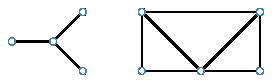
\includegraphics[scale=1.2]{Fig0.pdf}
	\caption{Esquema de las gráficas $G(4,3,3)$ (izquierda) y $G(5,7,1)$ (derecha).\label{F1}}
\end{figure}

\begin{theorem}
	Sea $G$ una gráfica clan crítica tal que su gráfica de clanes es $K_3$, entonces $G$ es la gráfica $G(4,3,3)$ ó $G(5,7,1)$.
\end{theorem}
\begin{proof}
Sea $G$ una gráfica clan crítica tal que $K(G)=K_3$. Al ser $K(G)=K_3$ entonces existen $q_1,q_2,q_3$ clanes de $G$, representados como los vértices de $K_3$. Cada par de clanes se interseca en al menos un vértice de $G$, es decir
\begin{equation*}
q_i\cap q_j\neq \emptyset, \quad \forall i,j\in\{1,2,3\},\quad i\neq j.
\end{equation*}
A continuación se muestra que existe un vértice $u_1$ de $G$, en el que se intersecan necesariamente los tres clanes de $G$, es decir $\{u_1\}\subset q_1\cap q_2 \cap q_3$. 

Supongamos que no existe un vértice $u_1$ que pertenezca simultáneamente a los tres clanes, es decir  $q_1\cap q_2 \cap q_3=\emptyset$. Bajo este supuesto, cada intersección $q_i\cap q_j$, $i\neq j$, contiene al menos un vértice, pero no hay un vértice común a todos. Sea $x_{ij}\in q_{i}\cap q_{j}$. Entonces $\{x_{12},x_{13},x_{23}\}$ forman una completa que se puede extender a un clan $q$. El clan $q$ es diferente de $q_{1},q_{2},q_{3}$ (pues, por ejemplo, $x_{23}\in q$ pero $x_{23}\not\in q_{1}$ por la condición de que $q_{1}\cap q_{2}\cap q_{3}=\emptyset$), lo cual contradice que $G$ sólo tenía los tres clanes $q_{1},q_{2},q_{3}$. 
Por lo tanto, necesariamente debe existir al menos un vértice $u_1$ tal que
\begin{equation*}
\{u_1\}\subset q_1\cap q_2 \cap q_3.
\end{equation*}
Para mostrar una igualdad estricta entre dichos conjuntos se sigue el siguiente argumento.

Supongamos existen $n$ vértices en dicha intersección de los tres clanes, con $n>1$. Con lo cual estos $n$ vértices pertenecen a cada uno de los clanes, es decir $\{v_1, \dots , v_n\} \subset q_i$ con $i\in\{1,2,3\}$. Sin embargo, esto implicaría que dichos vértices son adyacentes entre sí, formando una completa que se puede extender a un clan $q$ en $G$, lo que contradice el hecho de que solo existen tres clanes en $G$, pues $q$ es distinto a cada uno de los clanes $q_{1},q_{2},q_{3}$, pues en principio los clanes $q_{1},q_{2},q_{3}$ están constituidos por más de $n$ vértices. Por lo tanto se satisface 
\begin{equation*}
	\{u_1\}=q_1\cap q_2 \cap q_3.
\end{equation*}

En busca de saber qué gráfica es $G$, consideramos las intersecciones que pueden tener los clanes, con lo cual, resultan los siguientes casos a tratar, los cuales están considerando el hecho de la existencia del vértice $u_1$.
\begin{itemize}
\item Caso 1. 
Cualesquiera dos clanes de $G$ se intersecan únicamente en el vértice $u_1$, es decir $q_1\cap q_2\cap q_3=\left\{u_1\right\}$, $(q_1\cap q_3)\setminus q_2=\emptyset  \text{, }(q_2\cap q_3)\setminus q_1=\emptyset$ y $(q_1\cap q_2)\setminus q_3=\emptyset$, como se muestra en la figura~\ref{F2}.

\begin{figure}[!htbp]
	\centering
	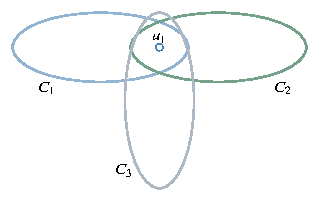
\includegraphics[scale=1.2]{Fig1.pdf}
	\caption{Esquema de los clanes de la gráfica $G$ correspondiente al caso 1.\label{F2}}
\end{figure}
Supongamos el clan $q_1$ está constituido por $n$ vértices, con $n>2$, de esta manera gráfica $G$ no cumpliría la condición de ser clan crítica, pues resultaría que $K(G)=K(G-\hat{u})$, para cualquier $\hat{u}\in q_1$, $\hat{u}\neq u_1$. Este razonamiento es aplicable para los clanes $q_2,q_3$, por lo tanto cada clan consta únicamente de dos vértices, con lo cual la gráfica $G=G(4,3,3)$.


\item Caso 2.
Existe una intersección dos a dos entre los clanes, de más de un vértice, considerando el vértice $u_1$. Sin pérdida de generalidad, supongamos que el clan $q_3$ interseca al clan $q_1$, así como a $q_2$, por demostrar
\begin{equation}\label{E1.1}
\left\{u_2\right\}=(q_1\cap q_3)\setminus q_2 \quad \text{y} \quad \left\{u_3\right\}=(q_2\cap q_3)\setminus q_1.
\end{equation}
Como se muestra en la figura~\ref{F3}. Sin embargo se sigue de manera inmediata que por el lema~\ref{L1.15} es correcta la expresión \eqref{E1.1}, pues el conjunto de vértices que están en $q_i\cap q_3$, $i=\{1,2\}$, y en ningún otro clan debe constar de cuando mucho un solo vértice, a dicho vértice se le etiqueto como $u_2,u_3$ respectivamente.

\begin{figure}[!htbp]
	\centering
	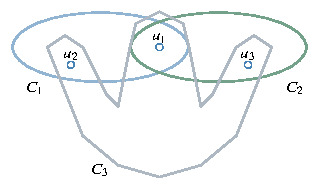
\includegraphics[scale=1.2]{Fig2.pdf}
	\caption{Esquema de los clanes de la gráfica $G$ correspondiente al caso 2.\label{F3}}
\end{figure}

A continuación demostraremos que los clanes $q_1$ y $q_2$ no pueden ser tales que están constituidos únicamente de dos vértices. 
Supongamos que $|q_1|=2$ y $|q_2|=2$, con lo cual $\left\{\left\{u_2,u_1\right\},\left\{u_1,u_3\right\},\left\{u_2,u_3\right\}\right\}\subset E(G)$, de esta manera, se formaría un nuevo clan distinto a $q_1,q_2$ y $q_3$, lo que contradiría la hipótesis de $K(G)=K_3$, pues existirían cuatro vértices en $K(G)$ y no tres. Como los clanes $q_1$ y $q_2$ no pueden tener solo dos vértices, deben tener al menos tres y no más pues se busca que la gráfica sea clan crítica, con lo cual se buscan clanes con menor cantidad de vértices posibles.
Siguiendo este razonamiento, se puede concluir que $|q_1|=|q_2|=|q_3|=3$, lo que da lugar a la gráfica $G=G(5,7,1)$.


\item Caso 3.
Los clanes de $G$ se intersecan en el vértice $u_1$ y sólo existe otra intersección entre dos de estos clanes. Sin pérdida de generalidad, supongamos que los clanes $q_1$ y $q_3$ se intersecan en un vértice $u_2$ de $G$ y $(q_2\cap q_3)\setminus q_1=\emptyset $, como se muestra en la figura~\ref{F4}.

\begin{figure}[!htbp]
	\centering
	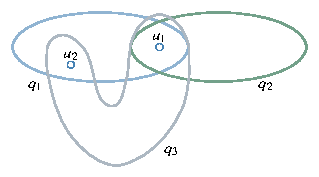
\includegraphics[scale=1.2]{Fig3.pdf}
	\caption{Esquema de los clanes de la gráfica $G$ correspondiente al caso 3.\label{F4}}
\end{figure}

Veamos que los clanes $q_1,q_3$ están constituidos únicamente por tres vértices. Pues si alguno de estos clanes tuviera menos de tres vértices, entonces existiría un vértice $\hat{u}$ en $q_1$ ó $q_3$ cuya eliminación no cambiaría la estructura de $K(G)$, lo que contradice la definición de clan crítica.

Por otro lado, consideremos $u_3\in V(q_3)$ tal que $u_3\neq u_1,u_2$. El clan $q_2$ debe estar constituido de más de dos vértices, pues de no ser así, consideremos un nuevo vértice $\hat{u}\neq u_1$ en $q_2$, ver figura~\ref{F5}.

\begin{figure}[!htbp]
	\centering
	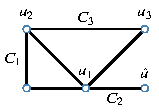
\includegraphics[scale=1.2]{Fig4.pdf}
	\caption{Esquema de los vértices y clanes de la gráfica $G$ correspondiente al caso 3, suponiendo que $q_2$ cuenta únicamente con dos vértices.\label{F5}}
\end{figure}

En tal caso se cumple que $K(G-u_2)=K(G)$, situación que no es válida. Con lo cual $|q_2|>2$ y se consideran los siguientes dos casos.
\begin{itemize}
\item Caso 3.1.
El vértice $u_3\notin V(q_2)$, entonces para todo $\overline{u}\in V(q_2)\setminus\{u_1\}$ se tiene que $K(G-\overline{u})=K(G)$, lo que implica que este caso no es posible, pues la eliminación de cualquier vértice de $q_2$, excepto $u_1$, no provoca un cambio en la estructura de $K_3$, lo que contradiría la hipótesis de clan crítica.

\item Caso 3.2.
El vértice $u_3\in V(q_2)$. Este caso se reduce al caso 2, con lo cual $G=G(5,7,1)$.
\end{itemize}
\end{itemize}
Resulta entonces que $G$ es la gráfica $G(4,3,3)$ ó $G(5,7,1)$.
\end{proof}


En el siguiente teorema se consideran las gráficas $G(3)$ y $G(4)$ que denotan el camino compuesto de tres y cuatro vértices respectivamente, ver figura~\ref{F6}.

\begin{figure}[!htbp]
	\centering
	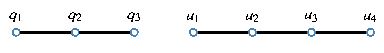
\includegraphics[scale=1.2]{Fig5.pdf}
	\caption{Esquema de las gráficas $G(3)$ (izquierda) y $G(4)$ (derecha), con sus respectivas etiquetas de acuerdo a sus vértices.\label{F6}}
\end{figure}

\begin{theorem}\label{T1.12}
Sea $G$ una gráfica clan crítica tal que su gráfica de clanes es $G(3)$, entonces $G$ es la gráfica $G(4)$.
\end{theorem}

\begin{proof}
Sea $G$ una gráfica clan crítica tal que $K(G)=G(3)$. La igualdad anterior implica directamente que existen únicamente tres clanes $q_1$, $q_2$ y $q_3$ tal que $q_1\cap q_3=\emptyset$. Dichos clanes están representados como los vértices de $G(3)$, ver figura~\ref{F6}.
Notemos que el clan $q_2$ tiene intersección no vacía con $q_1$ y $q_3$. A continuación se muestra un argumento con el cual es posible afirmar que en las intersecciones $q_1\cap q_2$ y $q_3\cap q_2$ constan únicamente de un vértice $u_2$ y $u_3$ de $G$, respectivamente.

Supongamos que existen $n$ vértices $\{v_1,\dots,v_n\}$ en $q_1\cap q_2$ con $n>1$, con lo cual se cumplen las siguientes contenciones $\{v_1,\dots,v_n\}\subset q_1 $ y $\{v_1,\dots,v_n\}\subset q_2$, lo que implica que los vértices $\{v_1,\dots,v_n\}$ son mutuamente adyacentes entre sí, lo que formaría una completa, y al extenderla un nuevo clan $q$ de $G$, de esta manera no se cumpliría que su gráfica de clanes fuese $G(3)$, pues tendría más de tres vértices su gráfica de clanes, dado que $q$ es distinto a $q_{1},q_{2}$ (existiría por ejemplo un vértice $v_{23}\in q_2\cap q_3$ que no esté en $q_1$, pues $q_1\cap q_3=\emptyset$, implicando que tampoco está en $q$), esta contradicción viene del hecho de suponer la existencia de $n$ vértices en $q_1\cap q_2$ con $n>1$, con lo cual tiene que ser $n=1$. Por lo tanto se satisface que 
\begin{equation*}
\{u_2\}=q_1\cap q_2.
\end{equation*}
Con un razonamiento análogo, se demuestra que de igual manera se satisface que 
\begin{equation*}
	\{u_3\}=q_3\cap q_2.
\end{equation*}

Por otra parte, lo que sigue es un razonamiento que demuestra que el clan $q_1$ está constituido de solo dos vértices, el ya mencionado $u_2$ y uno más en G; de igual manera el clan $q_3$ está constituido por el mencionado vértice $u_3$ y uno más en $G$. Demostraremos estos hechos para el caso del clan $q_1$, pues como anteriormente sucedió, el caso para la demostración del clan $q_3$ resultará análogo a la prueba del $q_1$. 


Así pues, consideremos que el clan $q_1$ está constituido por más de dos vértices, digamos $V(q_1)=\{v_1,\dots v_n\}$. Por ser un clan $q_1$, resulta que si retiramos un vértice $v_i$ de $q_1$, resulta que lo obtenido es una completa que se extiende a un clan también, para cualquier $i\in \{1,\dots,n\}$, con lo cual, al retirar cualquier vértice de $q_1$, excepto $u_2$, no modifica la estructura de su gráfica de clanes, lo que contradiría la hipótesis de ser $G$ clan crítica. Por lo tanto se requiere que $q_1$ tenga la menor cantidad de vértices posibles y que siga siendo un clan, por lo tanto sólo consta de dos vértices, $u_2$ y uno más $u_1$. De esta manera, también $q_3$ consta únicamente de dos vértices, $u_3$ y uno más $u_4$.

De acuerdo con el razonamiento planteado anteriormente, el clan $q_2$ también debe de constar únicamente de dos vértices, pues de ser más, se contradice la hipótesis de ser $G$ clan crítica de igual manera. Con lo cual, se puede concluir que $G$ es un camino de cuatro vértices, es decir, $G=G(4)$.
\end{proof}

El siguiente teorema es una generalización del teorema anterior, se consideran las gráficas $G(n-1)$ y $G(n)$, que denotan el camino compuesto por $n-1$ vértices y $n$ vértices, respectivamente. Ver figura~\ref{F7}.

\begin{figure}[!htbp]
	\centering
	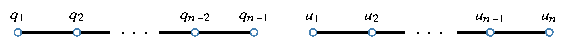
\includegraphics[scale=1.2]{Fig6.pdf}
	\caption{Esquema de las gráficas $G(n-1)$ (izquierda) y $G(n)$ (derecha), con sus respectivas etiquetas de acuerdo a sus vértices.\label{F7}}
\end{figure}

\begin{theorem}
Sea $G$ una gráfica clan crítica tal que su gráfica de clanes es $G(n-1)$, entonces $G$ es la gráfica $G(n)$.
\end{theorem}

\begin{proof}
Por hipótesis $K(G)=G(n-1)$, lo que implica que en $G$ existen $n-1$ clanes diferentes, que satisfacen $q_{k-1}\cap q_{k+1}=\emptyset$ para $k\in\{2,\dots n-2\}$; que representan los vértices de $G(n-1)$, como se muestra en la figura~\ref{F7} (izquierda).

Notemos que cada vértice en $G(n-1)$, que representa un clan de $G$, es adyacente con el vértice inmediato anterior y el inmediato siguiente. En el caso del primer vértice, adyacente con el inmediato siguiente; y en el caso del último vértice, adyacente con el inmediato anterior. Esto es que las intersecciones $q_1\cap q_2$, $q_2\cap q_3$, $\dots$ , $q_{n-3}\cap q_{n-2}$, $q_{n-2}\cap q_{n-1}$ son no vacías. Utilizando el mismo razonamiento expuesto en el teorema~\ref{T1.12}, se muestra que cada una de estas intersecciones es un único vértice, es decir
\begin{equation*}
\begin{aligned}
q_1\cap q_2 &= \{u_2\} \\
q_2\cap q_3 &= \{u_3\} \\
\vdots \\
q_{n-3}\cap q_{n-2} &= \{u_{n-2}\} \\
q_{n-2}\cap q_{n-1} &= \{u_{n-1}\}.
\end{aligned}
\end{equation*}

Por otra parte, se demostrará que el clan $q_1$ está constituido de solo dos vértices, el ya mencionado $u_2$ y uno más en G; de igual manera el clan $q_{n-1}$ está constituido por el mencionado vértice $u_{n-1}$ y uno más en $G$. Demostraremos estos hechos para el caso del clan $q_1$, pues el caso para la demostración del clan $q_{n-1}$ resultará análogo a la prueba del $q_1$. 

Consideremos que el clan $q_1$ está constituido por más de dos vértices, es decir $V(q_1)=\{v_1,\dots v_n\}$. Por ser un clan $q_1$, si retiramos un vértice $v_i$ de $q_1$, resulta que lo obtenido es una completa que se extiende a un clan también, para cualquier $i\in \{1,\dots,n\}$, con lo cual, al retirar cualquier vértice de $q_1$, excepto $u_2$, no modifica la estructura de su gráfica de clanes, lo que contradiría la hipótesis de ser $G$ clan crítica, por lo tanto sólo consta de dos vértices, $u_2$ y uno más $u_1$, pues de esta manera al retirar dicho vértice $u_1$, su gráfica de clanes sería distinta a $G(n-1)$, cumpliendo las hipótesis de ser clan crítica. 
De esta manera, también $q_{n-1}$ consta únicamente de dos vértices, $u_{n-1}$ y uno más $u_n$.

De acuerdo con el razonamiento planteado anteriormente, los clanes $q_2$, $q_3$, $\dots$ , $q_{n-3}$, $q_{n-2}$ también deben de constar únicamente de dos vértices, pues de ser más, se contradice la hipótesis de ser $G$ clan crítica, como se mostró. Con lo cual, se puede concluir que $G$ es un camino de $n$ vértices, es decir, $G=G(n)$.
\end{proof}

El siguiente teorema hace referencia la relación que existe entre la gráfica $G(6,6,18)$ y el árbol $T(4,2)$, extraídos del apéndice de gráficas y de diagramas de árbol en \cite{Harary:1969}, respectivamente. Dichas gráficas pueden verse en la figura~\ref{F8}

\begin{figure}[!htbp]
	\centering
	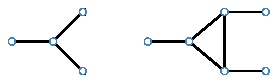
\includegraphics[scale=1.2]{Fig7.pdf}
	\caption{Esquema de las gráficas $T(4,2)$ (izquierda), con las etiquetas de sus vértices, y $G(6,6,18)$ (derecha).\label{F8}}
\end{figure}

\begin{theorem}
Sea $G$ una gráfica clan crítica tal que su gráfica de clanes es $T(4,2)$, entonces $G$ es la gráfica $G(6,6,18)$.
\end{theorem}

\begin{proof}
Sea $G$ una gráfica clan crítica tal que su gráfica de clanes es $T(4,2)$. Con lo cual, la gráfica $G$ debe tener cuatro clanes $q_1$, $q_2$, $q_3$ y $q_4$, representados como los vértices de $T(4,2)$, como se muestra en la figura~\ref{F8} (izquierda). Por las características de la gráfica de clanes de $G$, los clanes satisfacen que $q_1\cap q_3=\emptyset$, $q_1\cap q_4=\emptyset$ y $q_3\cap q_4=\emptyset$, además el clan $q_2$ tiene intersección no vacía con todos los demás.

El siguiente razonamiento concluye que la intersección que existe entre $q_2$ con cada uno de los demás clanes consta de un sólo vértice. Resulta que la prueba de dicha afirmación es análoga para $q_1,q_3,q_4$ con $q_2$, con lo cual se demostrará en el caso cuando se considera la intersección $q_1\cap q_2$.

Sea $u_{23}\in q_2\cap q_3$. Supongamos que en $q_1\cap q_2=\{v_1, \dots ,v_n\}$, es decir, existen $n$ vértices en la intersección, con $n>1$. Con lo cual se satisface $\{v_1, \dots ,v_n\}\subset q_1$ y $\{v_1, \dots ,v_n\}\subset q_2$, de esta manera $\{v_1, \dots ,v_n\}$ son mutuamente adyacentes, forman una completa, que se puede extender a un clan $q$ de $G$ distinto a los cuatro ya contemplados, pues por ejemplo $u_{23}\in q_2$ pero $u_{23}\notin q_1\cap q_2$, con lo cual $u_{23}\notin q$ y así $q\neq q_2$, de la misma manera se verifica inmediatamente que $q\neq q_1$, $q\neq q_3$ y $q\neq q_4$; lo que contradiría la hipótesis de que $K(G)=T(4,2)$, pues existirían al menos cinco clanes. Dicha contradicción viene del hecho de suponer que $n>1$, con lo cual $n=1$ y $q_1\cap q_2$ consta únicamente de un vértice, es decir
\begin{equation*}
q_1\cap q_2= \{u_2\}.
\end{equation*}
Por lo tanto, de igual manera se satisface que 
\begin{equation*}
\begin{aligned}
q_3\cap q_2 &= \{u_3\}, \\
q_4\cap q_2 &= \{u_4\}.
\end{aligned}
\end{equation*}

Los vértices $u_2$, $u_3$ y $u_4$, son distintos, pues de no serlo, las propiedades de $K(G)$ $q_1\cap q_3=\emptyset$, $q_1\cap q_4=\emptyset$ y $q_3\cap q_4=\emptyset$ no se satisfacerían. Este hecho implica que en $q_2$ existen al menos tres vértices, y en realidad, existen solo esos tres vértices, pues de existir más, no se cumpliría que $G$ fuese clan crítica, pues cualquier eliminación de vértices, que no sea $u_2$, $u_3$, $u_4$; no cambiaría la estructura de su gráfica de clanes.
De manera análoga, se demostrará que $q_1$, $q_3$ y $q_4$ constan únicamente de dos vértices. Supongamos que $q_1=\{v_1, \dots ,v_n\}$ con $n>2$. Bajo este supuesto, se cumpliría la igualdad $K(G)=K(G-v_i)$ con $v_i\in q_1$ y $v_i\neq u_2$, lo que implicaría que $G$ es no clan crítica. La contradicción proviene de suponer que $n>2$, por lo tanto $n=2$. Como se dijo, de manera análoga se demuestra que $q_3$ y $q_4$ constan únicamente de dos vértices.

Por lo tanto la gráfica $G$ correspondiente es la gráfica $G(6,6,18)$.
\end{proof}

El siguiente teorema considera el árbol $T(5,3)$ expuesto en el apéndice de diagramas de árbol en \cite{Harary:1969} y la gráfica $G(8,10)$, que representa la gráfica de ocho vértices y diez aristas, formando un ciclo de cuatro vértices. Los esquemas de dichas gráficas se pueden ver en la figura~\ref{F9}.

\begin{figure}[!htbp]
	\centering
	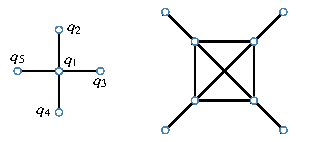
\includegraphics[scale=1.2]{Fig9.pdf}
	\caption{Esquema de las gráficas $T(5,3)$ (izquierda) y $G(8,10)$ (derecha).\label{F9}}
\end{figure}

\begin{theorem}
Sea $G$ una gráfica clan crítica tal que su gráfica de clanes es $T(5,3)$, entonces $G$ es la gráfica $G(8,10)$.
\end{theorem}

\begin{proof}
Sea $G$ una gráfica clan crítica tal que $K(G)=T(5,3)$, $K(G)$ tiene como vértices $q_1,q_2,q_3,q_4$ que representan los clanes de $G$, como se muestra en la figura~\ref{F9}. Dichos clanes cumplen las siguientes propiedades: el clan $q_i$, con $i\in \{2,3,4,5\}$, tiene intersección vacía con todos los clanes excepto con $q_1$, con lo cual la intersección de $q_1$ con cualquier clan es no vacía. 
A continuación se demostrará que cada una de estas intersecciones $q_1\cap q_i$ consta de un único vértice. La prueba es análoga para cada $i$, sin pérdida de generalidad consideraremos $i=2$, es decir, se demostrará que la intersección $q_1\cap q_2$ consta de un solo vértice $u_{12}$ y de esta manera concluir lo mismo con los demás clanes.

Sea $u_{13}\in q_1\cap q_3$. Supongamos que existen $n$ vértices en $q_1\cap q_2$ con $n>1$, es decir $q_1\cap q_2=\{v_1,\dots,v_n\}$. A partir de esto, se satisfacería que $\{v_1,\dots,v_n\}\subset q_1$ y $\{v_1,\dots,v_n\}\subset q_2$, por lo tanto dicho conjunto formaría una completa que se puede extender a un clan $q$ distinto a los demás clanes pues por ejemplo $u_{13}\in q_1$ pero $u_{13}\notin q_1\cap q_2$, con lo cual $u_{13}\notin q$ y así $q\neq q_1$, de la misma manera se verifica inmediatamente que $q$ es distinto a los demás clanes; lo que contradiría el hecho de que $K(G)=T(5,3)$ pues existirían al menos seis clanes. Dicha contradicción surge del hecho de considerar $n>1$, con lo cual $n=1$ y entonces
\begin{equation*}
q_1\cap q_2=u_{12}.
\end{equation*}
Como se dijo, de manera análoga, se concluye que 
\begin{equation*}
\begin{aligned}
	q_1\cap q_3 &= u_{13} \\
	q_1\cap q_4 &= u_{14} \\
	q_1\cap q_5 &= u_{15} .
\end{aligned}
\end{equation*}
Por el hecho que el clan $q_i$, con $i\in \{2,3,4,5\}$, tiene intersección vacía con todos los clanes excepto con $q_1$, los vértices anteriores son todos distintos.




\end{proof}




\bibliography{Ref}
\bibliographystyle{apalike}

\end{document}
